\documentclass{standalone}
\usepackage{tikz}
\usetikzlibrary{patterns, positioning}
\usepackage[sfdefault]{ClearSans} %% option 'sfdefault' activates Clear Sans as the default text font
\usepackage[T1]{fontenc}

\begin{document}
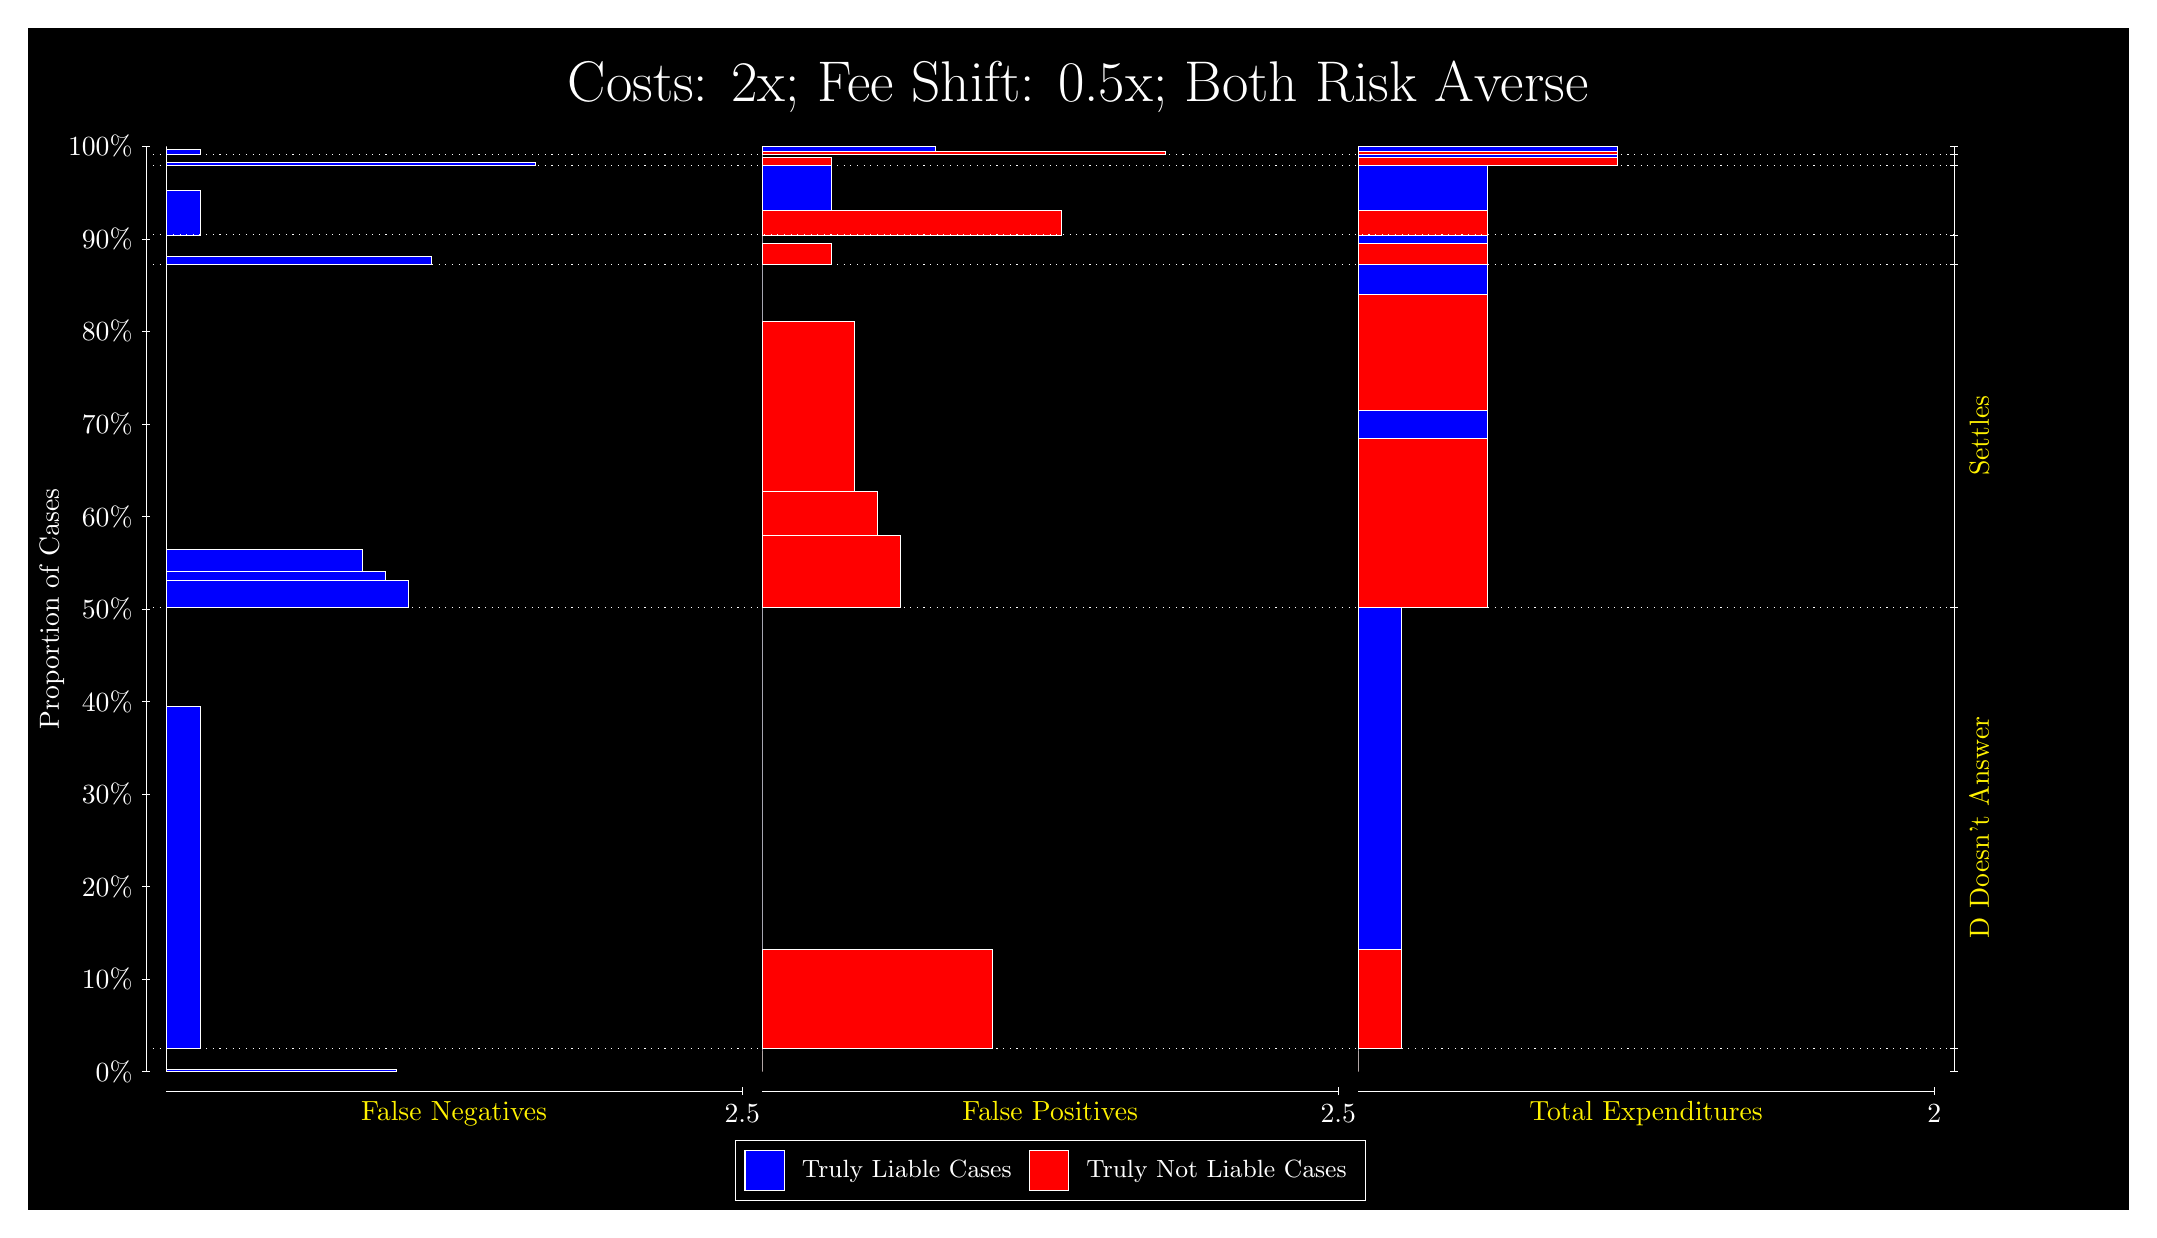
\begin{tikzpicture}
\draw[fill=black] (0,0) rectangle (26.667,15);
\draw[text=white] (0,13.5) rectangle (26.667,15) node[midway] {\huge Costs: 2x; Fee Shift: 0.5x; Both Risk Averse};
\draw[white, very thin] (1.5,1.75) -- (1.5,13.5);
\node[rotate=90, text=white, anchor=center] at (0.3, 7.625) {Proportion of Cases};
\draw[white, very thin] (1.45,1.75) -- (1.55,1.75);
\node[text=white, anchor=east] at (1.45, 1.75) {0\%};
\draw[white, very thin] (1.45,2.925) -- (1.55,2.925);
\node[text=white, anchor=east] at (1.45, 2.925) {10\%};
\draw[white, very thin] (1.45,4.1) -- (1.55,4.1);
\node[text=white, anchor=east] at (1.45, 4.1) {20\%};
\draw[white, very thin] (1.45,5.275) -- (1.55,5.275);
\node[text=white, anchor=east] at (1.45, 5.275) {30\%};
\draw[white, very thin] (1.45,6.45) -- (1.55,6.45);
\node[text=white, anchor=east] at (1.45, 6.45) {40\%};
\draw[white, very thin] (1.45,7.625) -- (1.55,7.625);
\node[text=white, anchor=east] at (1.45, 7.625) {50\%};
\draw[white, very thin] (1.45,8.8) -- (1.55,8.8);
\node[text=white, anchor=east] at (1.45, 8.8) {60\%};
\draw[white, very thin] (1.45,9.975) -- (1.55,9.975);
\node[text=white, anchor=east] at (1.45, 9.975) {70\%};
\draw[white, very thin] (1.45,11.15) -- (1.55,11.15);
\node[text=white, anchor=east] at (1.45, 11.15) {80\%};
\draw[white, very thin] (1.45,12.325) -- (1.55,12.325);
\node[text=white, anchor=east] at (1.45, 12.325) {90\%};
\draw[white, very thin] (1.45,13.5) -- (1.55,13.5);
\node[text=white, anchor=east] at (1.45, 13.5) {100\%};

\draw[white, very thin] (24.457,1.75) -- (24.457,13.5);
\draw[white, very thin] (24.407,1.75) -- (24.507,1.75);
\node[anchor=west] at (24.407, 1.75) {};
\draw[white, very thin] (24.407,2.0462) -- (24.507,2.0462);
\node[anchor=west] at (24.407, 2.0462) {};
\draw[white, very thin] (24.407,7.6464) -- (24.507,7.6464);
\node[anchor=west] at (24.407, 7.6464) {};
\draw[white, very thin] (24.407,12.003) -- (24.507,12.003);
\node[anchor=west] at (24.407, 12.003) {};
\draw[white, very thin] (24.407,12.375) -- (24.507,12.375);
\node[anchor=west] at (24.407, 12.375) {};
\draw[white, very thin] (24.407,13.256) -- (24.507,13.256);
\node[anchor=west] at (24.407, 13.256) {};
\draw[white, very thin] (24.407,13.396) -- (24.507,13.396);
\node[anchor=west] at (24.407, 13.396) {};
\draw[white, very thin] (24.407,13.5) -- (24.507,13.5);
\node[anchor=west] at (24.407, 13.5) {};

\draw[white, very thin, fill=blue] (1.75,1.75) rectangle (4.6775,1.7812);
\draw[white, very thin, fill=red] (1.75,1.7812) rectangle (1.75,2.0462);
\draw[white, very thin, fill=blue] (1.75,2.0462) rectangle (2.1891,6.39);
\draw[white, very thin, fill=red] (1.75,6.39) rectangle (1.75,7.6464);
\draw[white, very thin, fill=blue] (1.75,7.6464) rectangle (4.8239,7.9943);
\draw[white, very thin, fill=blue] (1.75,7.9943) rectangle (4.5312,8.1036);
\draw[white, very thin, fill=blue] (1.75,8.1036) rectangle (4.2384,8.3765);
\draw[white, very thin, fill=red] (1.75,8.3765) rectangle (1.75,12.003);
\draw[white, very thin, fill=blue] (1.75,12.003) rectangle (5.1167,12.103);
\draw[white, very thin, fill=red] (1.75,12.103) rectangle (1.75,12.375);
\draw[white, very thin, fill=blue] (1.75,12.375) rectangle (2.1891,12.941);
\draw[white, very thin, fill=red] (1.75,12.941) rectangle (1.75,13.256);
\draw[white, very thin, fill=blue] (1.75,13.256) rectangle (6.4341,13.297);
\draw[white, very thin, fill=red] (1.75,13.297) rectangle (1.75,13.396);
\draw[white, very thin, fill=blue] (1.75,13.396) rectangle (2.1891,13.459);
\draw[white, very thin, fill=red] (1.75,13.459) rectangle (1.75,13.5);
\draw[white, very thin, fill=red] (9.3189,1.75) rectangle (9.3189,2.015);
\draw[white, very thin, fill=blue] (9.3189,2.015) rectangle (9.3189,2.0462);
\draw[white, very thin, fill=red] (9.3189,2.0462) rectangle (12.246,3.3026);
\draw[white, very thin, fill=blue] (9.3189,3.3026) rectangle (9.3189,7.6464);
\draw[white, very thin, fill=red] (9.3189,7.6464) rectangle (11.075,8.5551);
\draw[white, very thin, fill=red] (9.3189,8.5551) rectangle (10.783,9.1211);
\draw[white, very thin, fill=red] (9.3189,9.1211) rectangle (10.49,11.273);
\draw[white, very thin, fill=blue] (9.3189,11.273) rectangle (9.3189,12.003);
\draw[white, very thin, fill=red] (9.3189,12.003) rectangle (10.197,12.275);
\draw[white, very thin, fill=blue] (9.3189,12.275) rectangle (9.3189,12.375);
\draw[white, very thin, fill=red] (9.3189,12.375) rectangle (13.125,12.69);
\draw[white, very thin, fill=blue] (9.3189,12.69) rectangle (10.197,13.256);
\draw[white, very thin, fill=red] (9.3189,13.256) rectangle (10.197,13.355);
\draw[white, very thin, fill=blue] (9.3189,13.355) rectangle (9.3189,13.396);
\draw[white, very thin, fill=red] (9.3189,13.396) rectangle (14.442,13.437);
\draw[white, very thin, fill=blue] (9.3189,13.437) rectangle (11.515,13.5);
\draw[white, very thin, fill=red] (16.888,1.75) rectangle (16.888,2.015);
\draw[white, very thin, fill=blue] (16.888,2.015) rectangle (16.888,2.0462);
\draw[white, very thin, fill=red] (16.888,2.0462) rectangle (17.437,3.3026);
\draw[white, very thin, fill=blue] (16.888,3.3026) rectangle (17.437,7.6464);
\draw[white, very thin, fill=red] (16.888,7.6464) rectangle (18.534,9.7983);
\draw[white, very thin, fill=blue] (16.888,9.7983) rectangle (18.534,10.146);
\draw[white, very thin, fill=red] (16.888,10.146) rectangle (18.534,11.621);
\draw[white, very thin, fill=blue] (16.888,11.621) rectangle (18.534,12.003);
\draw[white, very thin, fill=red] (16.888,12.003) rectangle (18.534,12.275);
\draw[white, very thin, fill=blue] (16.888,12.275) rectangle (18.534,12.375);
\draw[white, very thin, fill=red] (16.888,12.375) rectangle (18.534,12.69);
\draw[white, very thin, fill=blue] (16.888,12.69) rectangle (18.534,13.256);
\draw[white, very thin, fill=red] (16.888,13.256) rectangle (20.181,13.355);
\draw[white, very thin, fill=blue] (16.888,13.355) rectangle (20.181,13.396);
\draw[white, very thin, fill=red] (16.888,13.396) rectangle (20.181,13.437);
\draw[white, very thin, fill=blue] (16.888,13.437) rectangle (20.181,13.5);
\draw[white, dotted] (1.5,2.0462) -- (24.457,2.0462);
\draw[white, dotted] (1.5,7.6464) -- (24.457,7.6464);
\draw[white, dotted] (1.5,12.003) -- (24.457,12.003);
\draw[white, dotted] (1.5,12.375) -- (24.457,12.375);
\draw[white, dotted] (1.5,13.256) -- (24.457,13.256);
\draw[white, dotted] (1.5,13.396) -- (24.457,13.396);
\draw[white, very thin] (1.75,1.5) -- (9.0689,1.5);
\node[text=yellow, anchor=north] at (5.4094, 1.5) {False Negatives};
\draw[white, very thin] (9.0689,1.45) -- (9.0689,1.55);
\node[text=white, anchor=north] at (9.0689, 1.45) {2.5};

\draw[white, very thin] (9.3189,1.5) -- (16.638,1.5);
\node[text=yellow, anchor=north] at (12.978, 1.5) {False Positives};
\draw[white, very thin] (16.638,1.45) -- (16.638,1.55);
\node[text=white, anchor=north] at (16.638, 1.45) {2.5};

\draw[white, very thin] (16.888,1.5) -- (24.207,1.5);
\node[text=yellow, anchor=north] at (20.547, 1.5) {Total Expenditures};
\draw[white, very thin] (24.207,1.45) -- (24.207,1.55);
\node[text=white, anchor=north] at (24.207, 1.45) {2};


\node[text=yellow, centered, rotate=90] at (24.777, 4.8463) {D Doesn't Answer};
\node[text=yellow, centered, rotate=90] at (24.777, 9.8248) {Settles};





\draw (12.978300999999998,1.5) node[draw=none] (baseCoordinate) {};
\begin{scope}[align=center]
        \matrix[scale=0.5, draw=white, below=0.5cm of baseCoordinate, nodes={draw}, column sep=0.1cm]{
            \node[rectangle, draw, minimum width=0.5cm, minimum height=0.5cm, fill=blue] {}; &
            \node[draw=none, font=\small, text=white] (B) {Truly Liable Cases}; &
            \node[rectangle, draw, minimum width=0.5cm, minimum height=0.5cm, fill=red] {}; &
            \node[draw=none, font=\small, text=white] (B) {Truly Not Liable Cases}; \\
            };
\end{scope}

\end{tikzpicture}
\end{document}